\documentclass[prb,preprint]{revtex4-1} 

\usepackage{amsmath}  
\usepackage{amsfonts} 
\usepackage{graphicx} 
\usepackage{color}
\begin{document}


\title{Franck-Hertz Experiment\textcolor{red}{;}\textcolor{green}{:} Measuring Transition Energies of Neon and Mercury}

\author{Jiajun Shi}
\email{jshi15@amherst.edu} 
\affiliation{Department of Physics, Amherst College, Amherst, MA, 01002}


\author{Danika Luntz-Martin}
\email{dluntzma@smith.edu}
\affiliation{Department of Physics, Smith College, Northampton, MA , 01063}


\date{\today}

\begin{abstract}

We recreated the canonical Franck-Hertz experiment and measured the energy required to excite neon and mercury atoms.  \textcolor{blue}{Hey! What happened to the key discovery F-H made, and why they received the Nobel prize? That is, you didn't just measure the energy required (which could equally well describe an experiment on a classical as well as a quantum system), you more importantly demonstrated that the energy levels in atoms are QUANTIZED. That should be in your lead sentence! }  

\textcolor{blue}{Be more specific in the next sentence (some suggestions in magenta):} Using a\textcolor{magenta}{n applied} voltage \textcolor{magenta}{varying/ranging/spanning from 0 - 100? V, up to 100? V, or similar language} we accelerated electrons through a gas of either neon or mercury atoms \textcolor{blue}{you did both, so consider rephrasing to something like}\textcolor{magenta}{ `first neon, then mercury' or `a gas of the element under study' or similar}. 
\textcolor{blue}{OK, but why? you try to address that later, of course, but adding a short little phrase like the following (not particularly artfully worded) example to the end of the previous sentence would clarify your PURPOSE and METHOD right away instead of guessing how the second sentence in your abstract is related to the first sentence:}\textcolor{magenta}{   `...gases of various elements so as to study when collisions between the electrons and the gas molecules would result in energy transfers to the atoms' or perhaps `how much kinetic energy an electron needed to acquire before it had enough energy to promote an atom to its next highest energy level' or 'your wording here' }

\textcolor{blue}{This next paragraph is a bit confusing. Phrases like `the number of electrons... decrease' wrongly suggests that electrons are disappearing, instead of just slowing down when they collide inelastically with gas atoms (thereby transferring part of their kinetic energy to the atoms). A drop in current doesn't mean a decrease in the number of electrons in the system, it means a decrease in their speed (because of a decrease in kinetic energy).  }
We measured the electron current reaching the anode. As we increased the magnitude of the accelerating voltage we saw the number of electrons reaching the anode decrease to a minimum at evenly spaced intervals. The drops in the electron current were caused by electron obtaining enough energy, from the accelerating voltage, to cause the neon or mercury atoms to reach an excited state. After the colliding inelasticity with an atom the electrons did not have enough energy to reach the anode resulting the drop in electron current. By measuring the difference between the minima in the electron current we were able determine the excitation energy of neon. \textcolor{blue}{isn't this true of Hg as well?}

Mercury has an optimal temperature \textcolor{red}{were} the number of minima is maximized and their amplitude is still discernible. After determining  the optimum temperature range with direct measurements of electron current, we used a lock-in detector to get more precise measurements of the minima. 

We plotted the difference in energy \textcolor{magenta}{against the number of the minimum}\textcolor{blue}{what does `the number of the minimum' mean?} and \textcolor{magenta}{used fit lines to extrapolate to a minimum number of .5.} \textcolor{blue}{huh? An abstract needs to ``stand alone.'' That is, it needs to make sense on its own, even if you don't read the rest of the paper.  No one reading the abstract will understand why you would do this particular extrapolation or what a minimum number of 0.5 means. Since what is really important is that this is method of using this information (your measurements) to infer the energy of the first excited state in Hg (or perhaps the first two???) after correcting for }\textcolor{magenta}{ something }\textcolor{blue}{ involving mean free path --- }\textcolor{magenta}{you get to chose the more specific wording to replace 'something' }\textcolor{blue}{--- why not say that? }  Averaging all of our data we got excitation energy for neon of 18.5 $\pm$ .4 \textcolor{red}{V} and for mercury of 4.58 $\pm$ .4 \textcolor{red}{V}. \textcolor{red}{Volt is not a unit of energy. eV is a unit of energy. 'electron volts' are not volts, they are energies, just as} $(1.609 \cdot 10^{-19}C)(18.5 V) = 29.8 \cdot 10^{-19}J$ \textcolor{red}{is a unit of energy (Joules). The difference between eV and J is that in eV units, the charge on an electron is} `1 e' \textcolor{red}{rather than }$1.609 \cdot 10^{-19}$ Coulomb. 

\textcolor{blue}{Remember that the abstract should stand alone. Therefore, don't leave the reader in suspense, give the actual values so they can compare theory and experiment without having to read the rest of the paper: } Our results for both mercury and neon agree with the expected values \textcolor{magenta}{of ? eV} for the excitation energies of neon and \textcolor{magenta}{of ? eV and ? eV for the first two excited states in } mercury. However neither of our values were precise enough to correspond to a single excitation energy because of the resolution of our instruments. \textcolor{blue}{is it possible you are seeing more than one excitation energy? could you be exciting atoms into the 1st and the 2nd excited states from the ground state? or to the first excited state from neutral atoms and also from ionized atoms?}

\end{abstract}


\maketitle 

\section{Introduction}
\label{introduction}

In 1913, Niels Bohr postulated that electrons within an atom can only occupy certain discrete energy levels in his famous Bohr model for atoms. This theory also requires any change in an electron's energy to be discontinuous as well, equaling to a difference between two of the energy levels. It was not until the next year, 1914, that James Franck and Gustav Hertz provided experimental \textcolor{red}{evidences to} Bohr's energy level postulation. In a vacuum chamber they designed to study the dynamics of the electrons passing through a vapor of mercury, Franck and Hertz observed that a collision between an electron and a mercury atom could result in the electron losing a specific amount of its kinetic energy. The electrons with exactly this amount of kinetic energy were completely decelerated and stopped during the collisions with the atoms, while the faster electrons kept moving forward after the collisions, but lost the same amount of kinetic energy. Slower electrons may collide with the mercury atoms as well, but they did not lose an appreciable amount of kinetic energy.  They also discovered that an electron could lose a multiple of this amount of energy when it passed through the vacuum chamber, \textcolor{blue}{provided that it is fast enough to endure this loss}. \textcolor{magenta}{more to the point, provided it had gained enough kinetic energy in between collisions}. 

Franck and Hertz's discovery was consistent with the Bohr model because the collision between an electron (unbound) and a mercury atom could transfer the kinetic energy of the unbound electron to the atom and excite a bound electron inside the atom from the lowest energy level to a higher one. The energy difference between these two energy levels was equal to the kinetic energy loss that occurs to the fast electrons. One should understand that although the Bohr model is regarded as a simplistic and insufficient interpretation of quantum mechanics, \textcolor{green}{its proposal of the bound electron's energy quantization nonetheless provided insights into the atom's internal structures}.\textcolor{magenta}{more to the point, its prediction of energy quantization remains true in more advanced models of quantum mechanics. As written, your sentence in green reads as if quantization isn't really true but is just an approximation. It is the model that is the approximation, not the existence of quantized energy levels! } 

\textcolor{blue}{very helpful:} Later on, Franck and Hertz published another paper about the emissions of light from the atoms that acquired energy from the collider electrons-- the excited electron inside the atom decayed into the lowest energy level, emitting a photon with frequency $\nu=E/h$, where E is the energy difference between the two levels, and $h$ is the Planck constant. The kinetic energy absorption and the photon emission jointly demonstrate the quantization of bound electron's energy levels.

Franck and Hertz's apparatus used a \textcolor{red}{transparent vacuum glass tube} \textcolor{blue}{do you mean a glass vacuum tube?} to contain the \textcolor{magenta}{wordy: experiment environment and enable visibility of the light emission patterns}.\textcolor{blue}{by `experiment environment' do you mean `gas?' by `enable visibility' do you mean `observe' or perhaps `see?'} A heated filament (cathode) was used to emit free electrons via thermionic emissions. The vacuum tube was heated, so the mercury inside turned into vapor and filled the entire vacuum tube. \textcolor{blue}{good description, but missing a key detail: the vapor pressure (and hence also the mean free path for electrons between collisions, which affects the amount of KE that can be gained between collisions) is temperature dependent. Since in some of your experiments you are going to vary the gas density and mean free path by varying temperature, you should mention this detail here.} There was a control grid, held at a distance from the filament, that was used to create an accelerating voltage. The electric field resulted from this accelerating voltage pulled the electrons towards the grid, and then further to an anode behind the grid to be collected. The anode was held at a voltage slightly negative to the accelerating grid to discourage the electrons that lost their kinetic energy from reaching the anode. Franck and Hertz changed the accelerating voltage and measured the current due to the electrons that reached the anode. They discovered that the current experienced several sharp drops at certain accelerating voltages. The spacings between the voltages of two adjacent drops were always approximately equal-- 4.9 V, meaning that an electron lost 4.9 eV of energy every time it collided with a mercury atom and excited a bound electron inside the atom from the ground level to a higher level. Franck and Hertz also discovered that the light emitted from the apparatus had wavelength 254nm, corresponding to exactly 4.9 eV of energy by $\nu=E/h$.

\textcolor{blue}{this reads as if you mixed the Ne and Hg atoms together in a single gas. See  green text for suggested replacements for red text}. We attempt to reproduce the Franck-Hertz experiment in \textcolor{red}{the}\textcolor{green}{this}  lab. We conduct \textcolor{red}{the experiment with both neon gas and mercury vapor}. \textcolor{green}{separate experiments with a gas of neon atoms and a gas of mercury atoms }. 

With the modern understanding of the atom's internal energy structure, we \textcolor{blue}{word choice: would} be able to find the exact energy level transition involved in the experiment. We use apparatuses similar to that of the original Franck-Hertz experiment, but with some modifications to improve signal-to-noise ratio that will be introduced in the next section. For both neon and mercury, we measure the currents based on varying accelerating voltages. In addition to the original Franck-Hertz experiment, we add temperature control to the apparatus for the mercury atom and study the temperature dependence of the internal transition of the mercury atom.However, in the mercury experiment, we encounter large uncertainties in our results, and to improve our measurements, we implement a lock-in technique for precision measurement of the voltage values where we have sharp drops in current.

\section{Methods}

We perform the Franck-Hertz experiment with two types of atoms-- neon and mercury. In each setup, we \textcolor{red}{DELETE ought to} bombard the atoms using electrons whose kinetic energy is controllable. We then can collect the electrons after they pass through the bombardment area, and measure the current due to this collection. The electrons are accelerated by a voltage we can control using a power supply. If we measure the current due to electron collection under different accelerating voltage values, we can find the electrons' final kinetic energy's (after bombardment) dependence on their initial kinetic energy.

\subsection{Neon Gas}

\textcolor{blue}{helpful and informative description of emission current:} We use a glass tube filled with neon gas at room temperature to perform the Franck-Hertz experiment. Fig \ref{figneon} shows an illustrative diagram of our setup. K is a filament that emits electrons when heated, and it serves as the cathode. The current through the filament is controlled by the power source $U_{F}$. We ought to hold this current invariant through out the experiment because it controls the rate of electron emissions, thus any variance in this current could introduce a shift in the final collected current. The current we use to hold constant and optimize the electron emission rate is 149 mA.

\begin{figure}
    \centering
    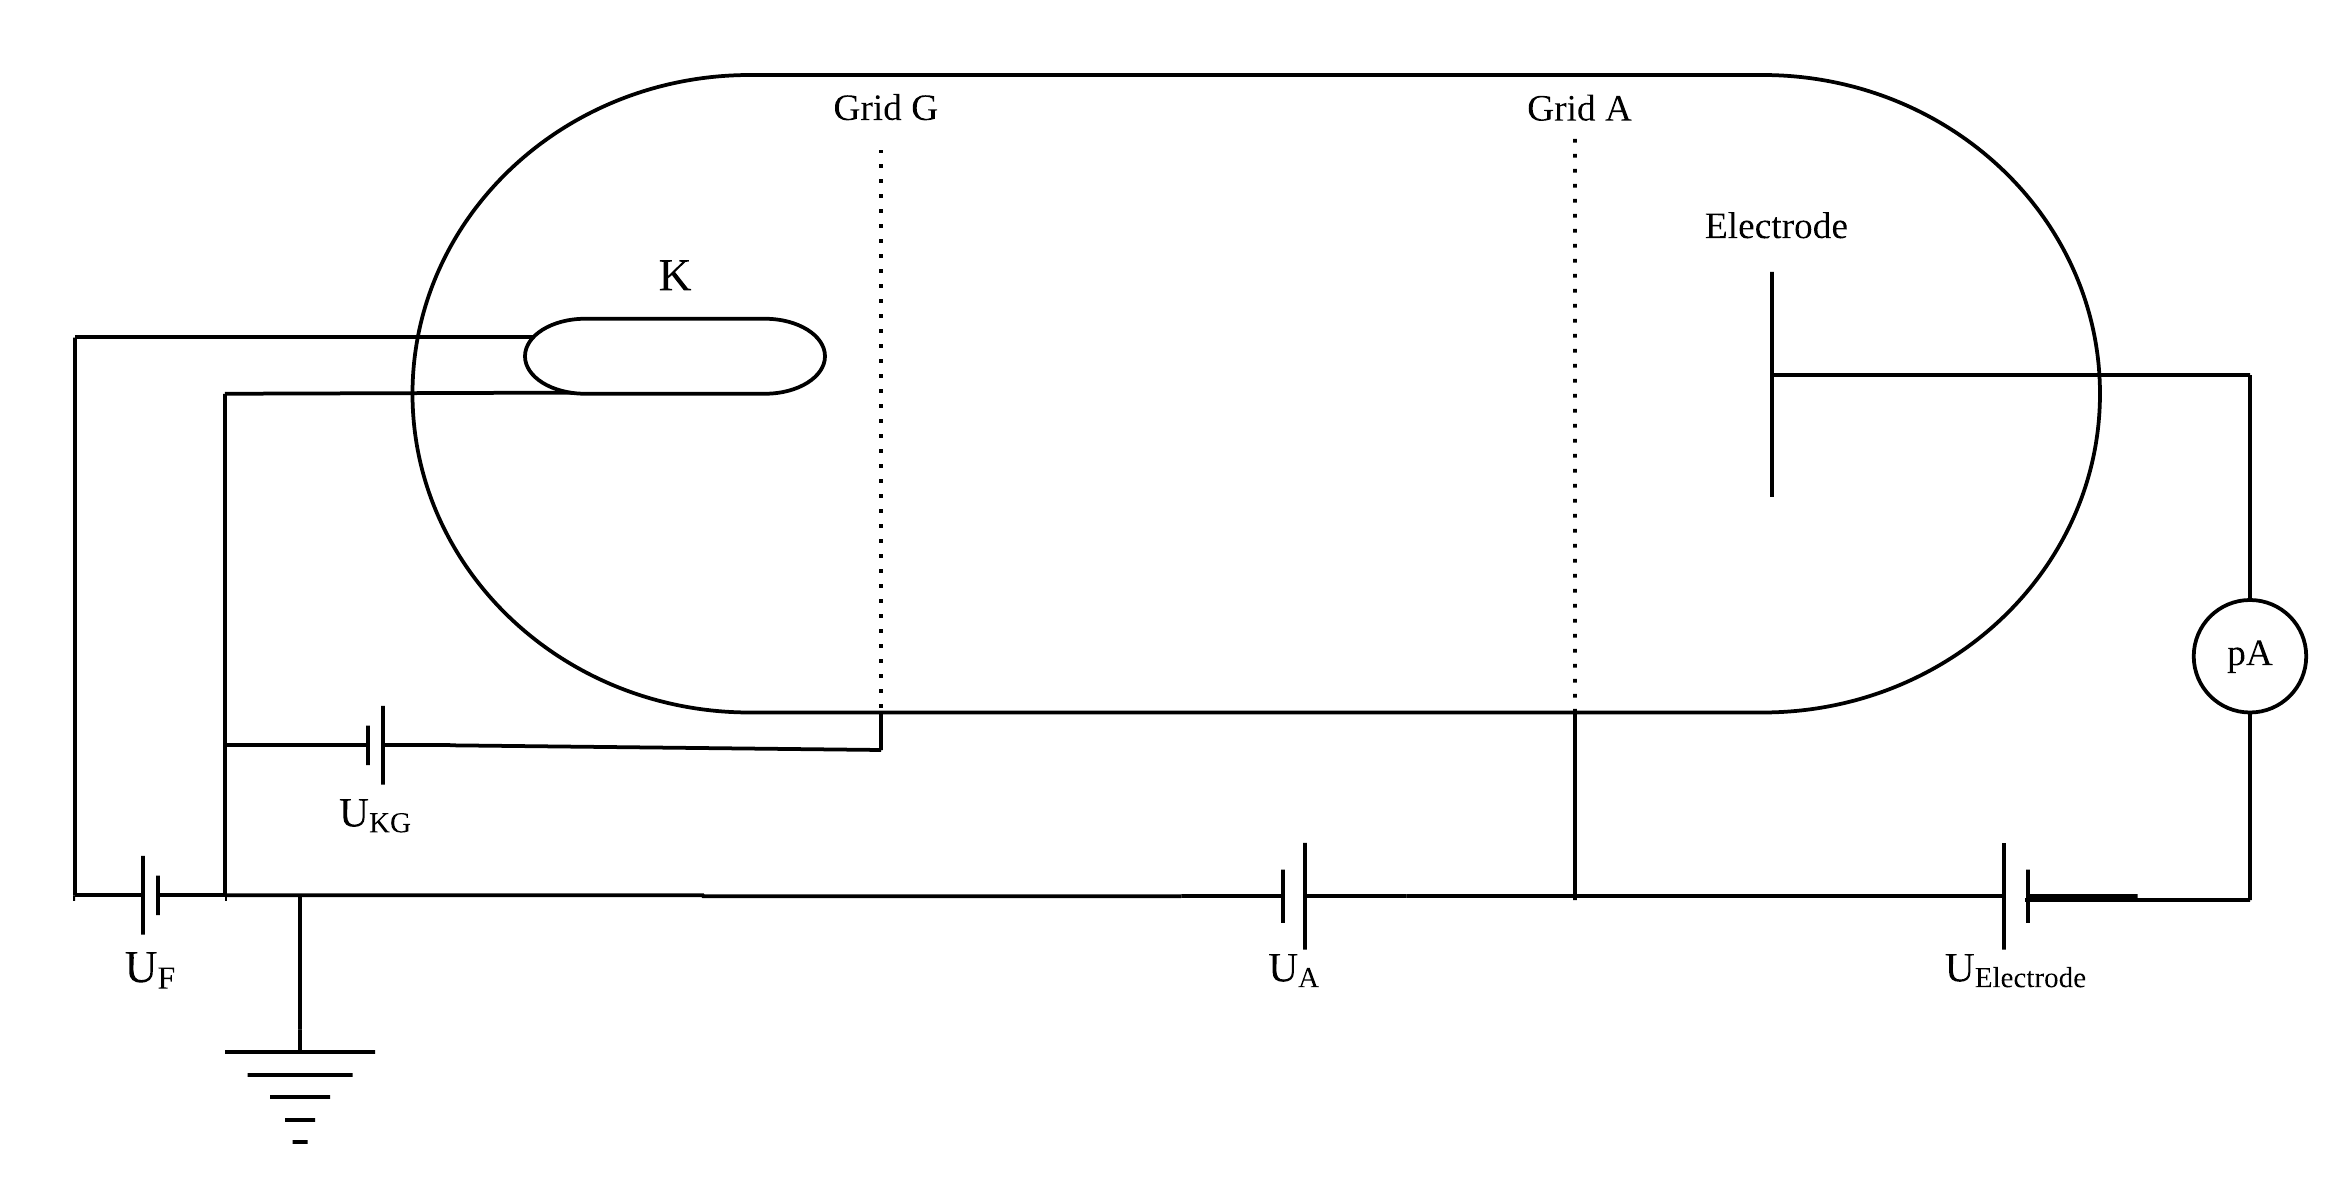
\includegraphics[width=\textwidth]{figneon.png}
    \caption{Experiment setup for the neon sample.}
    \label{figneon}
    \end{figure}

The emitted electrons from the filament may roam freely near the cathode, so \textcolor{red}{they we install} a grid G in the vicinity of the cathode and  applied \textcolor{magenta}{tenses of \textit{install} and \textit{applied} don't match} an initial accelerating voltage to it so that the electrons were drawn towards the grid. The voltage on grid G is held at 2.6 V through a power source $U_{KG}$. This initial preparation \textcolor{magenta}{awkward phrasing: makes the emitted electrons be effectively pulled by the field created by the the accelerating voltage}. Grid A is where the accelerating voltage is applied, by another source $U_{A}$, to make electrons acquire kinetic energy in an amount we can control. The accelerating voltage $U_{A}$ can be set as any value between 0 and 80 V, manually or by ramp control. Ramp control sweeps through the 0-80 V range 60 times a second.\textcolor{blue}{did you use this? why or why not? For example, too fast?} 

It is worth noticing that the voltage applied to grid G contributes to the acceleration of the electrons as well, so the total accelerating voltage in the tube is the sum of the two voltages. Behind grid A, there is an electrode serving to collect the electrons flying through grid A. This collector electrode has to be held at a voltage relatively negative to grid A. This way the electrons that lose all of their kinetic energy during collisions are unable to reach the collector, because we do not want those electrons to contribute to the current. \textcolor{blue}{why not?}

We have one multimeter measuring the accelerator voltage and another one measuring the current through the collector electrode. We \textcolor{red}{DELETE: ought to} control the power supply $U_{A}$ to increase the accelerating voltage. Initially we \textcolor{red}{color}{tense: attempt} to utilize ramp control to better resolve the change in the current due to the change in the accelerating voltage, but have to give up since the multimeters we use are not capable of effectively responding that fast. \textcolor{magenta}{yes, the 60 Hz sweep is an older technology designed for use with (analog) oscilloscopes}. Instead, we manually control the accelerating voltage and try to increase it as slowly as possible. The \textcolor{red}{result}\textcolor{blue}{need the \textit{adjective} form of \textit{result} here} current is plotted versus the \textit{accelerating} voltage.

\subsection{Mercury Vapor}

Performing the Franck-Hertz experiment on mercury requires slight modification to the apparatus. We use a similar glass tube to bombard the mercury atoms with accelerated electrons, but this time the mercury has to be vaporized first. Under room temperature, the mercury inside the tube is in its liquid state. To get enough mercury vapor, we need to heat the glass tube up to a relatively high temperature. We do not have to reach mercury's boiling point as all we need is a sufficient amount of mercury vapor to be bombarded by the electrons. This requirement in the mercury experiment prompts us to seek the optimal temperature to measure the current's dependence on voltage, so we will perform measurements under different temperatures. We will use an oven enclosing the whole glass tube to control the temperature.

\begin{figure}
    \centering
    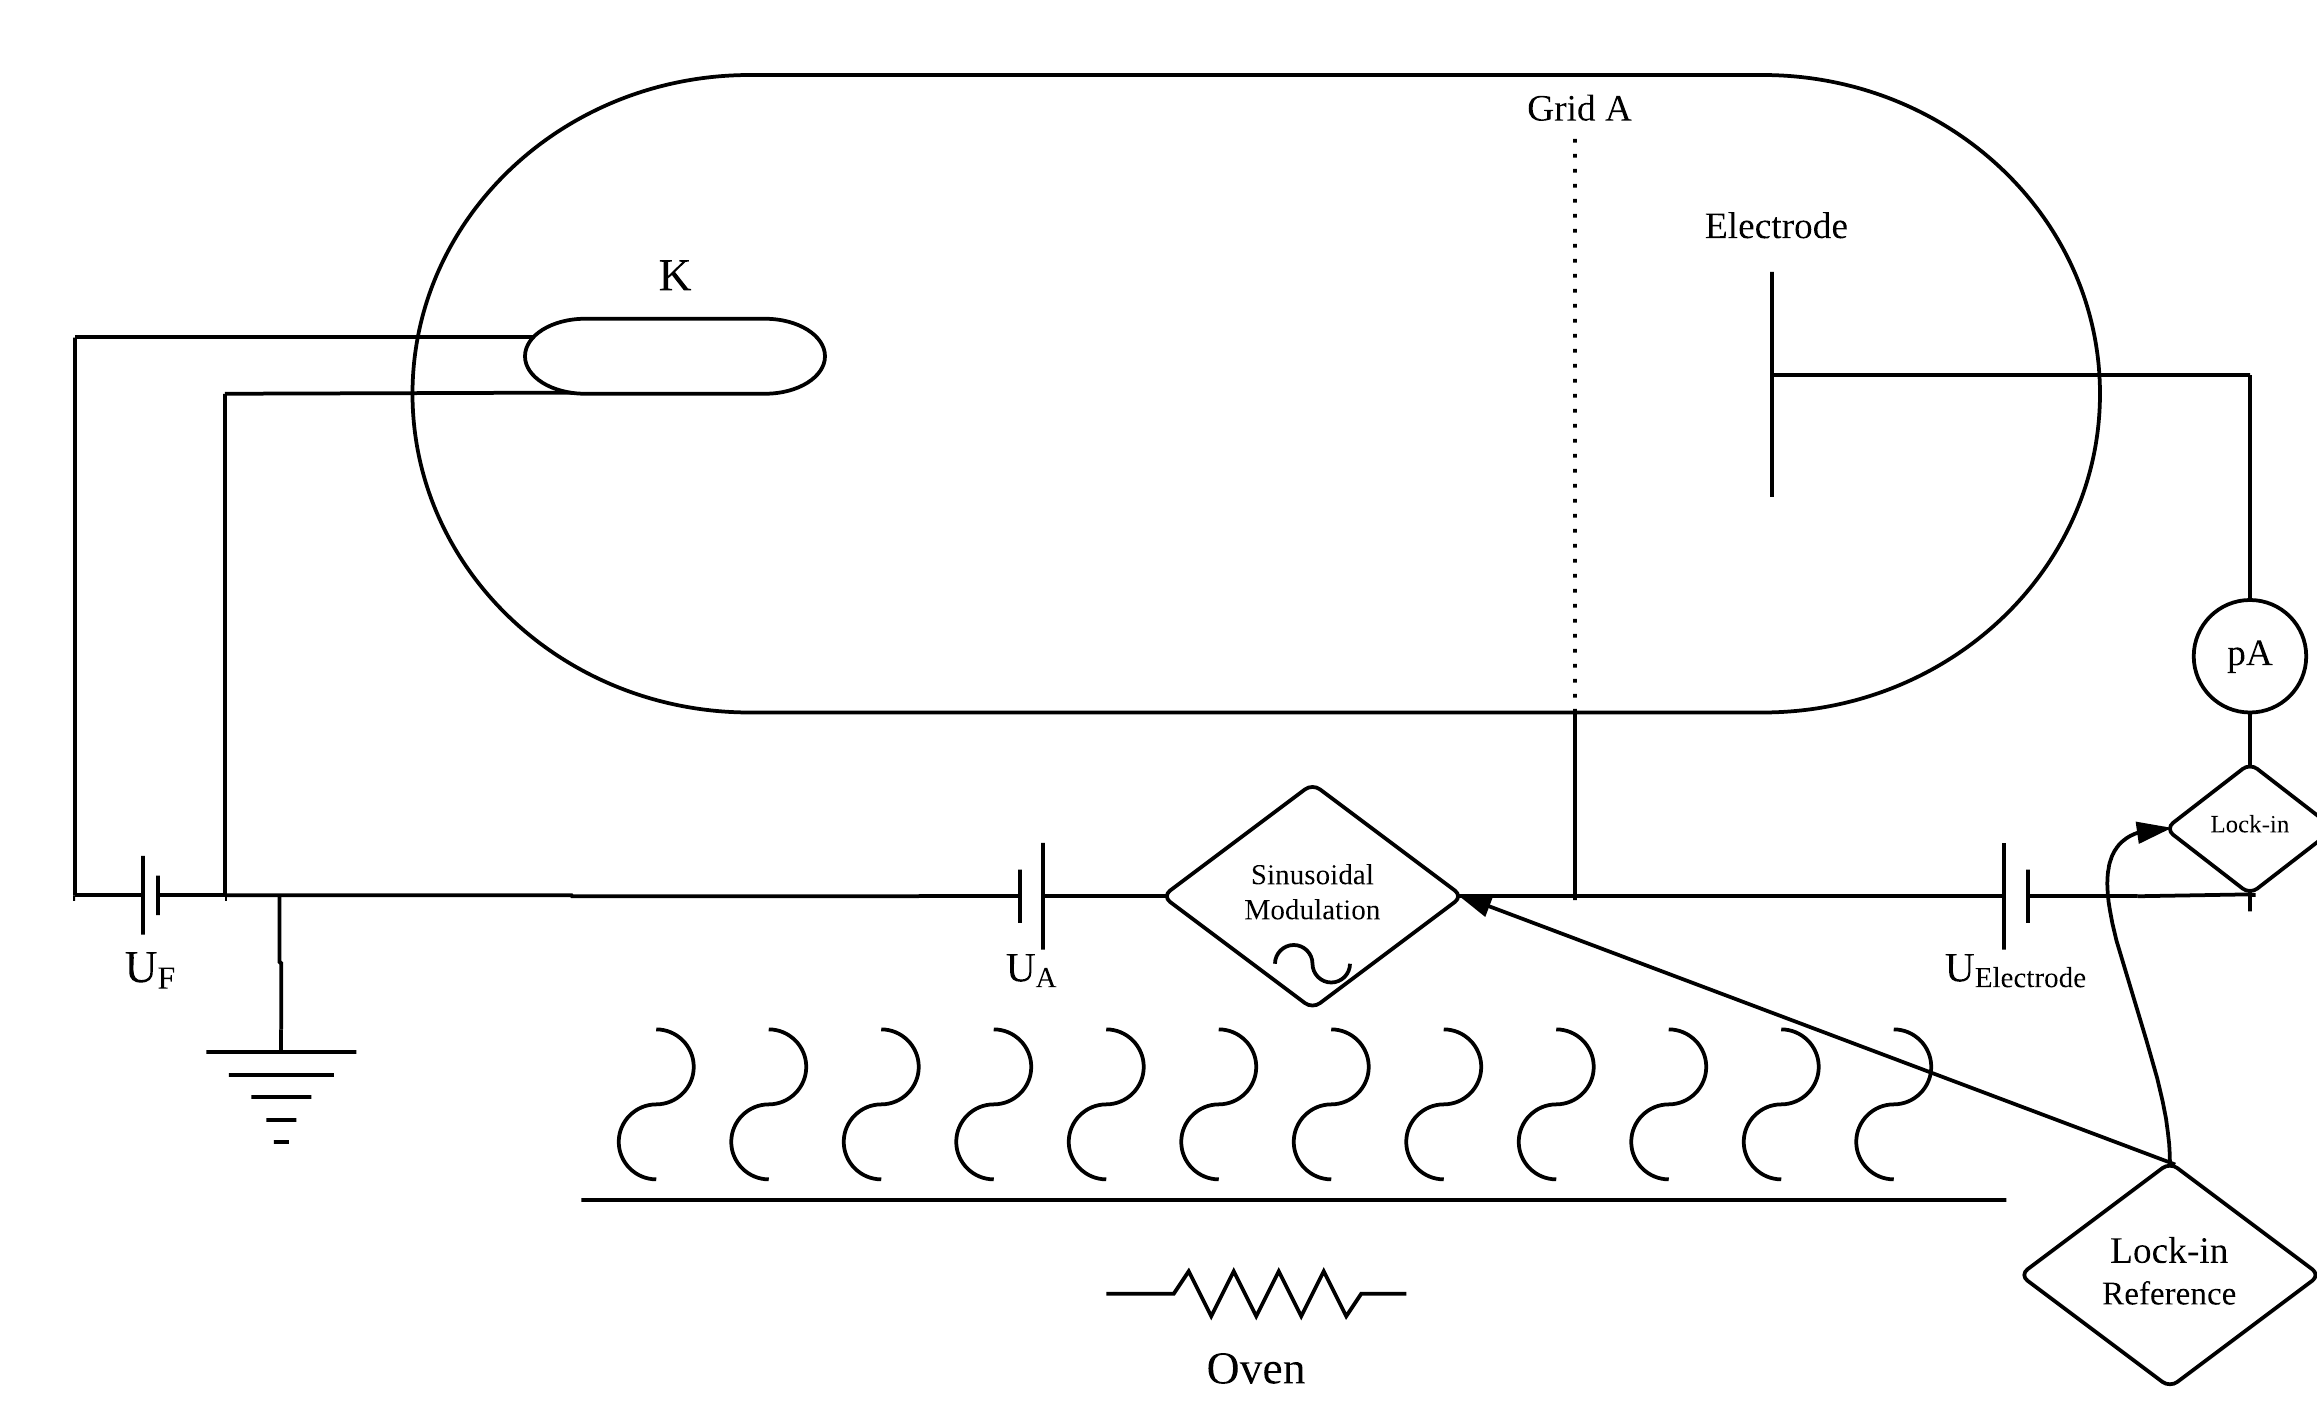
\includegraphics[width=\textwidth]{fighg.png}
    \caption{Experiment setup for the mercury sample. 
    \textcolor{blue}{even though the terms are described in the text, there should also be a short, abbreviated description of each labeled element in this figure. For example: Electrons are emitted from the filament K, then accelerated towards the electrode by .... Also define symbols such as }
    $U_F$, $U_A$ 
    \textcolor{blue}{etc}}
    \label{fighg}
    \end{figure}

As seen in Fig \ref{fighg}, the initial accelerating voltage is not present in this experiment. A voltage of 6.5 V is applied to the electron-emitting filament and is held constant throughout the experiment. \textcolor{blue}{why not a constant current, as with the Ne tube?} We still use an accelerator grid A to increase the electrons' kinetic energy. This time we can tune between 0 V and 70 V for the accelerating voltage. A retarding voltage of 1.5 V is applied to the collector electrode to serve the same purpose as in the neon example. We will again manually control the accelerating voltage to increase it as smoothly as possible. The results of the two experiments are presented in the next section.


\section{Results}

\subsection{Neon}

We did four data runs using neon. For each run we recorded the accelerating voltage (x data) and the electron current measured by the anode, this current was recorded as a voltage measured across an internal resistor (y data). Each of our runs showed three discernible minima in the voltage corresponding to electron current. These dips are the voltages just before the electrons have enough energy (from the accelerating voltage) to reach the anode even after an inelastic collision with a neon atom. In an attempt to be concise we are not showing all of our data, Figure~\ref{neon_data} is representative of all the data we collected. The apparent double minima, see the second and third dips in Figure~\ref{neon_data}, is most likely caused by by energy levels with very similar excitation energies.~\cite{newfeatures} \textcolor{blue}{can you separate these in your data? What are these expected energy levels? Later you only list one value}. Also of interest is the voltage corresponding to the steepest negative slope which is when the majority of electrons have enough energy to cite the neon atoms. However the location of the steepest negative slope was difficult to determine from our data as can be seen in Figure~\ref{neon_data}.

\textcolor{blue}{If I recall correctly, you could infer where the collisions were occuring by looking at the light emitted by neon atoms returning to the ground state after collision-induced excitations. This supports your argument in Fig 3 (and is also just plain neat!). You should mention this (and include a photo if you have one).}

\begin{figure}[h!]
\centering

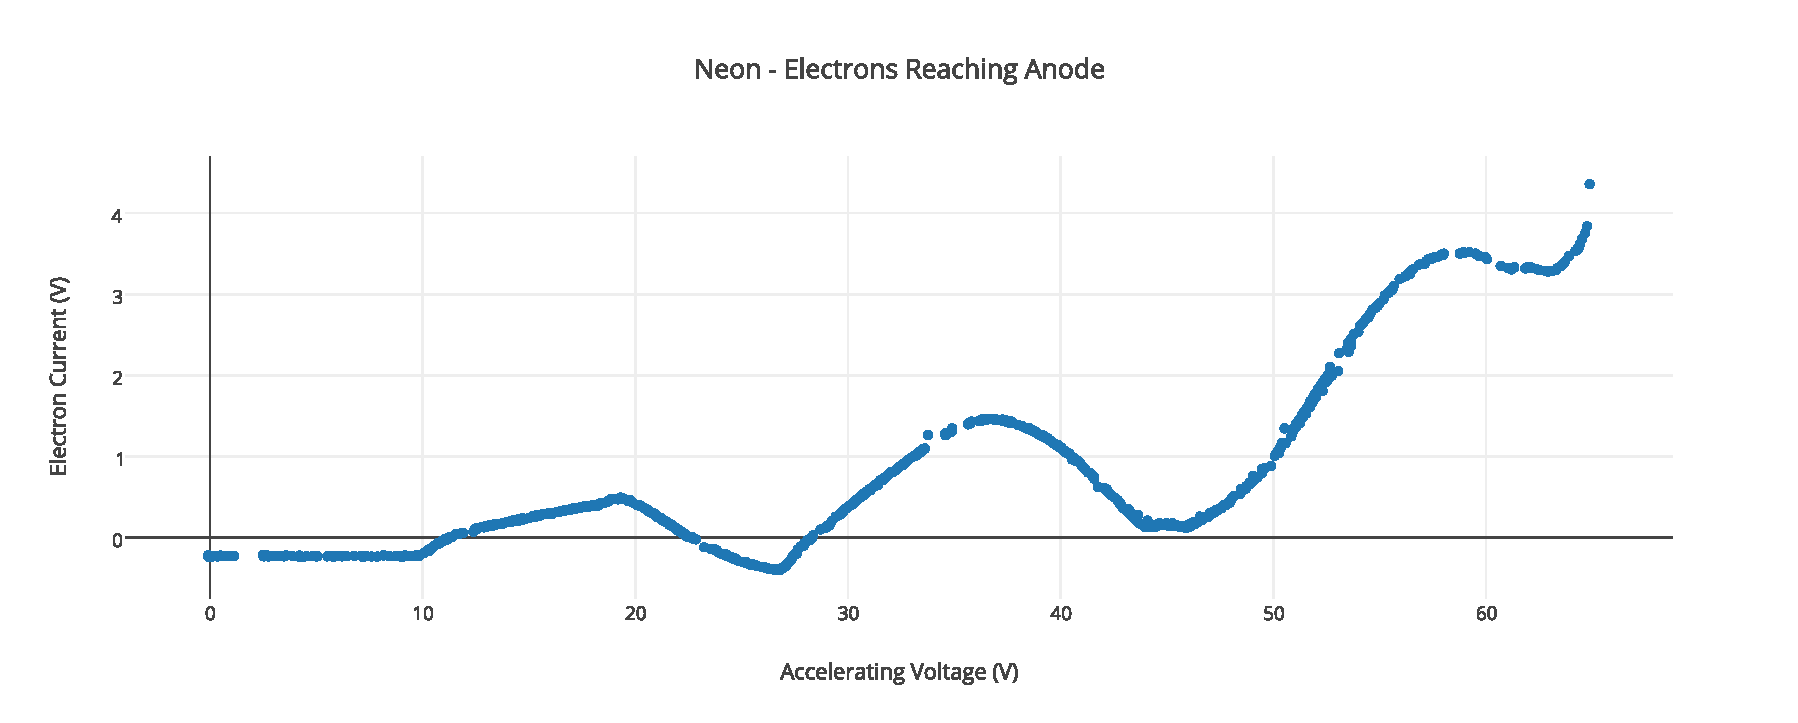
\includegraphics[width=6in]{neon_data.pdf}
\caption{Neon data with electron current as a voltage plotted against accelerating voltage. The three minima correspond to each electron exciting three neon atoms before reaching the anode. The double minima in the second and third dips is due to multiple excitation levels with similar energies.}



\label{neon_data}
\end{figure}


\subsection{Mercury}

Since the number of discernible dips for mercury depends on temperature, we collected data in 10$^{\circ}$C increments starting at 150$^{\circ}$C and ranging to 210$^{\circ}$C. From this data, see Figure~\ref{hg_data}, it can be seen that there is an optimum temperature at around 200$^{\circ}$C at which the most minima can be observed. 

\begin{figure}[h!]
\centering

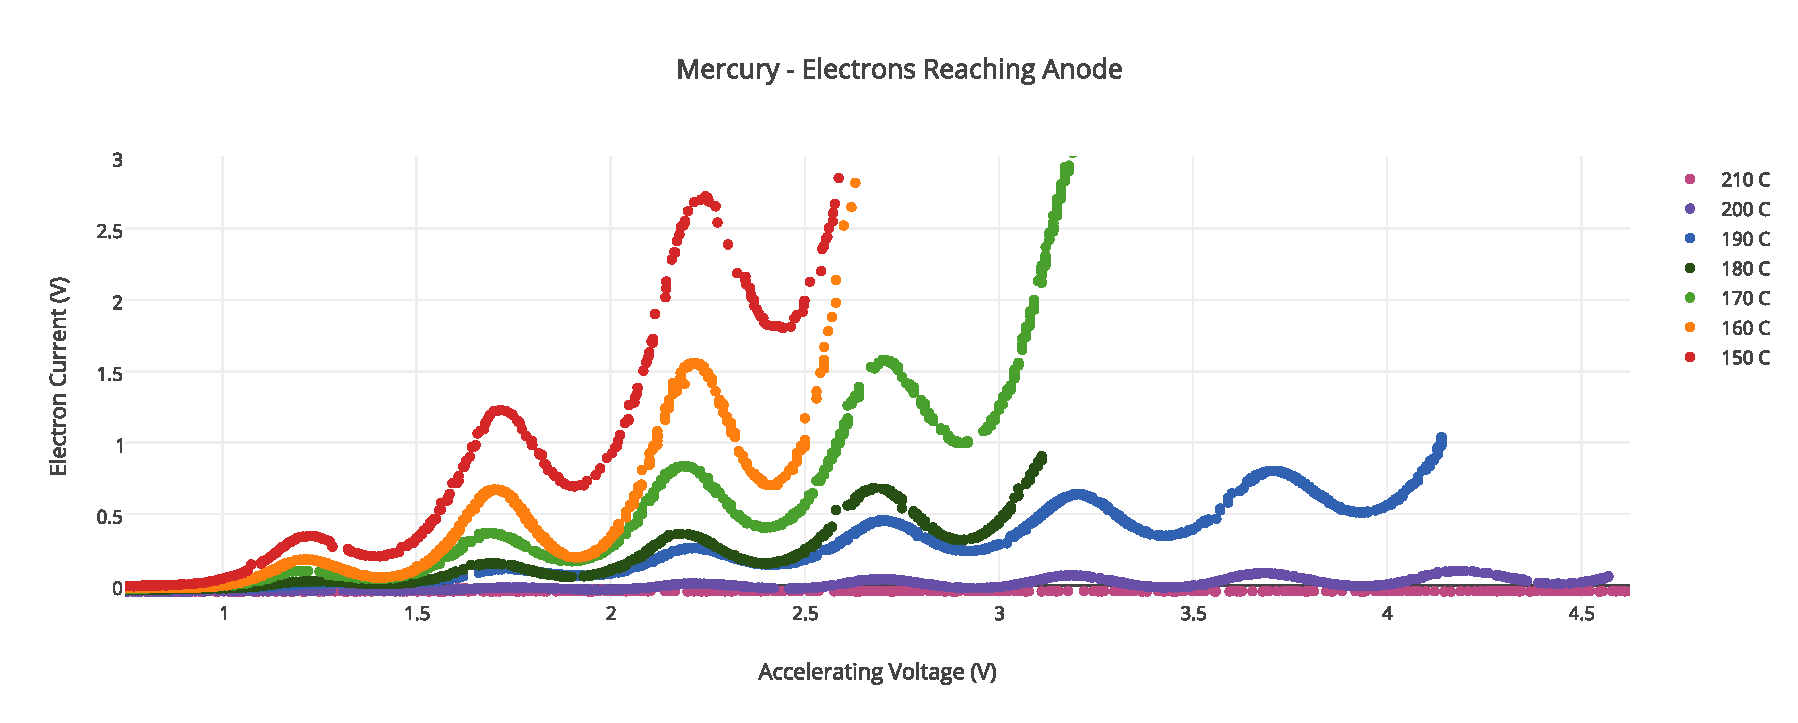
\includegraphics[width=6in]{hg_data.pdf}
\caption{Mercury data for temperatures ranging from 150$^{\circ}$C to 210$^{\circ}$C. The range of temperatures shows the optimum temperature to be approximately 190 - 200$^{\circ}$C. For higher temperatures, such as 210$^{\circ}$C, the minima in electron current are not discernible. For lower temperatures, for example 150$^{\circ}$C and 160$^{\circ}$C, there were fewer minima before the mercury atoms are ionized.}

\label{hg_data}
\end{figure}

Using the information that we obtained about the optimum range of temperature, we took a more data using a lock-in detector. \textcolor{blue}{if you used a lock-in amplifier, you must have modulated something to produce a time-varying signal at a particular frequency and phase. Explain what you modulated and how you did it. A circuit diagram --- some modified version of Fig 2, perhaps --- would also help with the explanation} The lock-in \textcolor{red}{this is confusingly worded: blocked the upward slope in electron current}, see particularly 150$^{\circ}$C in Figure~\ref{hg_data}. With the lock-in we took data from 185$^{\circ}$C to 215$^{\circ}$C in increments of 5$^{\circ}$C. The output from the lock-in, see Figure~\ref{hg_lockin}, is the derivative of the direct output without the lock-in. Therefore, the minima in the lock-in output correspond to the steepest negative slope of the direct output and the places the lock-in data passes through zero correspond to the minima and maxima of the direct output. The lock-in detector was highly sensitive to ionization of the mercury atoms. Our 185$^{\circ}$C data already showed significant reduction in the number of minima because of ionization. \textcolor{blue}{and at lower temperatures, better or worse? You provide an answer in the caption but it should also be here in the text.} Because of space considerations \textcolor{magenta}{what space considerations? please include the other data sweeps in an appendix if not shown here} we are not showing all of our lock-in data. Figure~\ref{hg_lockin} is the data collected for 205$^{\circ}$C and is a representative sample of the data collected.

\begin{figure}[h!]
\centering

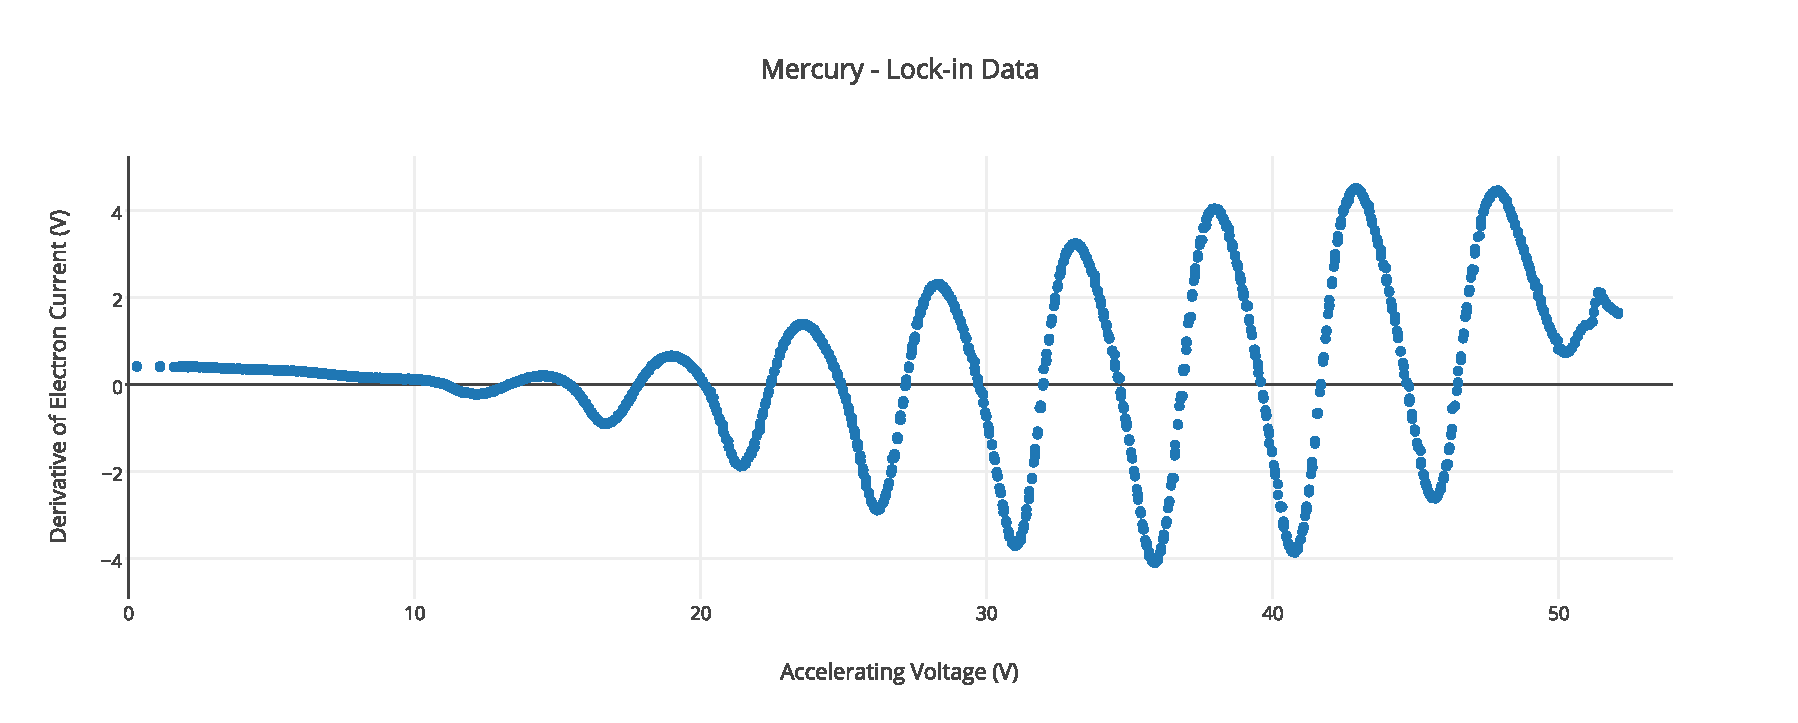
\includegraphics[width=6in]{hg_lockin.pdf}
\caption{Sample mercury data at 205$^{\circ}$C using the lock-in detector. The lock-in output is the derivative of the direct output in Figure~\ref{hg_data}. Minima in the voltage correspond to the steepest negative slope of the electron current and the lock-in x intercepts with positive slopes correspond to the minima in the direct output.}

\label{hg_lockin}
\end{figure}



\section{Analysis}

\subsection{Neon}

To determine the energy needed to excite the neon atoms we needed to find the spacing of the minima in electron current (which we measured as a voltage.) We visually determined the locations of the minima and the steepest negative slopes with uncertainty for each of our data runs, see sample data in Figure~\ref{neon_data}. We then calculated the change in voltage between adjacent minima and between adjacent steepest slopes. These values can be seen in Table~\ref{neon_dvs}.

\begin{table}[h!]
\centering
\caption{The difference in voltage for adjacent minima and adjacent steepest negative slopes obtained from all of data runs. Our best value is the average of these values. The large errors are from the difficulty in determining the location of minima and steepest slopes.}
\begin{ruledtabular}
\begin{tabular}{c c c c}
$\Delta$V Minima & Error $\Delta$V Minima & $\Delta$V Steepest Slope &  Error $\Delta$V Steepest Slope\\
\hline	% horizontal line to separate headings from data
19.0 & 2.0 & 19.2 & 1.5  \\
16.4 & 2.0 & 19.5 & 1.5  \\
18.5 & 1.3 & 20.0 & 2.5  \\
17.6 & 1.6 & 18.5 & 2.5  \\
18.4 & 1.2 & 19.5 & 2.0  \\
17.0 & 1.5 & 18.8 & 2.0  \\
18.5 & 1.5 & 18.5 & 2.5  \\
17.5 & 2.5 & 19.5 & 2.0  \\

\end{tabular}
\end{ruledtabular}
\label{neon_dvs}
\end{table}

We then averaged the first column and got 17.9 $\pm$ .3 eV as the average difference between the minima, where the uncertainty is the standard deviation of the mean. From the difference between the steepest slopes we got an average value of 19.19 $\pm$ .19 eV. We then averaged those two values, to get a final value of 18.5 $\pm$ .4 eV where uncertainty is again the standard deviation of the mean. This value agrees with our expectations because neon has a large number of transitions with energies ranging from 18.3 eV to 18.9 eV.

\subsection{Mercury}

Because of the temperature dependence of the mercury data, the process by which we found the energy level was more involved. We began our analysis in a similar way to our analysis of neon by visually determining the location of the minima and steepest negative slope. However, when we calculated the difference in voltage between minima this method gave us an uncertainty on the order of 10$\%$. We then plotted the distance between minima versus the minimum number as suggested by Rapior, Sengstock and Baev~\cite{newfeatures} and fit linear lines to the data for each temperature. Rapior, Sengstock and Baev found that the fit lines from each temperature converged toward the minima number .5. We found that the fit lines to our data did not converge at dip number .5, furthermore the uncertainty for our minima was large enough to make our results imprecise and unsatisfying.

To improve our results, we used that data collected using the lock-in detector. Because the lock-in output is the derivative of the direct output it is the x intercept with a positive slope that corresponds to the minima in the direct data and the minima of the lock-in output corresponds to the steepest negative slopes of the direct output. Figure~\ref{rel_error} shows the data from the direct output steepest slope and minima and the corresponding lock-in outputs (minima and positive slope x-intercept) for 200$^{\circ}$C. The data with the least uncertainty was that data from the lock-in using the positive x intercepts to calculate the differences in voltage. From this data we found the values seen in Table~\ref{hg_lockin_table}.

\begin{figure}[h!]
\centering

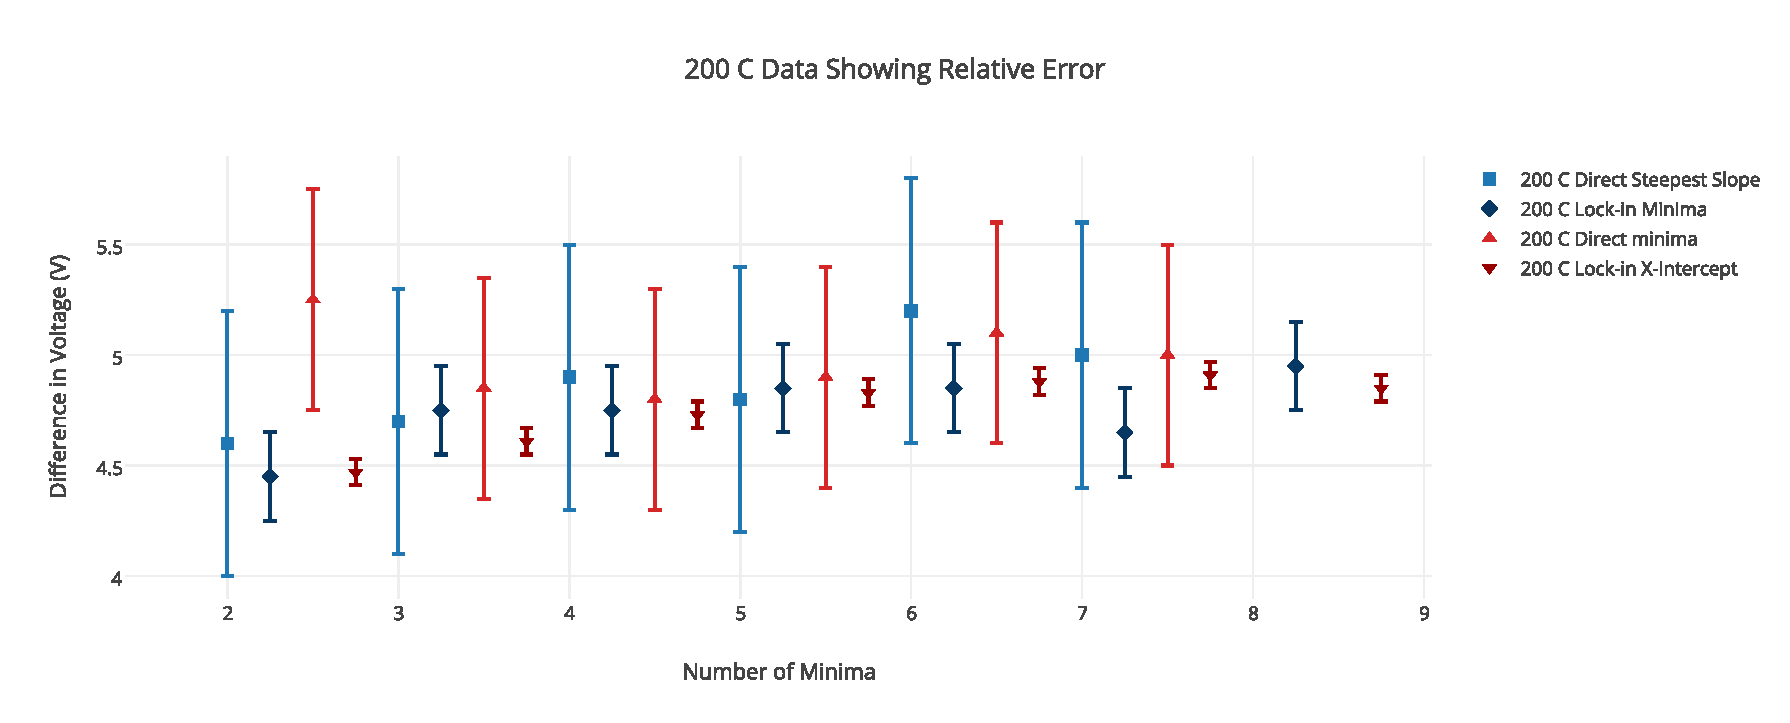
\includegraphics[width=6in]{rel_error.pdf}
\caption{All the 200$^{\circ}$C data shown with the relative errors. The blue data is the steepest negative slope from the direct data and the corresponding lock-in minima data. The lock-in data has less than half the error of the direct data. The red data is the direct output minima and the lock-in positive x-intercepts. The lock-in positive x-intercepts had the least uncertainty.}

\label{rel_error}
\end{figure}


\begin{table}[h!]
\centering

\caption{The difference in voltage for consecutive positive slope x-intercepts in from the lock-in output. The first dip was indiscernible for the 215$^{\circ}$C data and the higher minima of the 195$^{\circ}$C and 185$^{\circ}$C data were lost due to ionization. The error for these values is ~1.3$\%$}

\begin{ruledtabular}
\begin{tabular}{c c c c c c c c}
Dips & $\Delta$V 215$^{\circ}$C & $\Delta$V 210$^{\circ}$C  & $\Delta$V 205$^{\circ}$C &$\Delta$V 200$^{\circ}$C  & $\Delta$V 195$^{\circ}$C  & $\Delta$V 195$^{\circ}$C &$\Delta$V 185$^{\circ}$C  \\
\hline	% horizontal line to separate headings from data
1 - 2 &         & 4.67 & 4.53 & 4.42 & 4.36 & 4.58 & 4.51 \\
2 - 3 & 4.63 & 4.57 & 4.63 & 4.61 & 4.63 & 4.78 & 4.82 \\
3 - 4 & 4.67 & 4.69 & 4.63 & 4.73 & 4.84 & 4.87 & 4.90 \\
4 - 5 & 4.74 & 4.79 & 4.89 & 4.83 & 4.87 & 4.93 &         \\
5 - 6 & 4.76 & 4.80 & 4.87 & 4.88 & 4.95 & 4.99 &         \\
6 - 7 & 4.76 & 4.82 & 4.84 & 4.91 &         & 5.05 &         \\
7 -8  & 4.76 & 4.73 & 4.77 & 4.85 &         & 4.90 &         \\

\end{tabular}
\end{ruledtabular}
\label{hg_lockin_table}
\end{table}


\begin{figure}[h!]
\centering

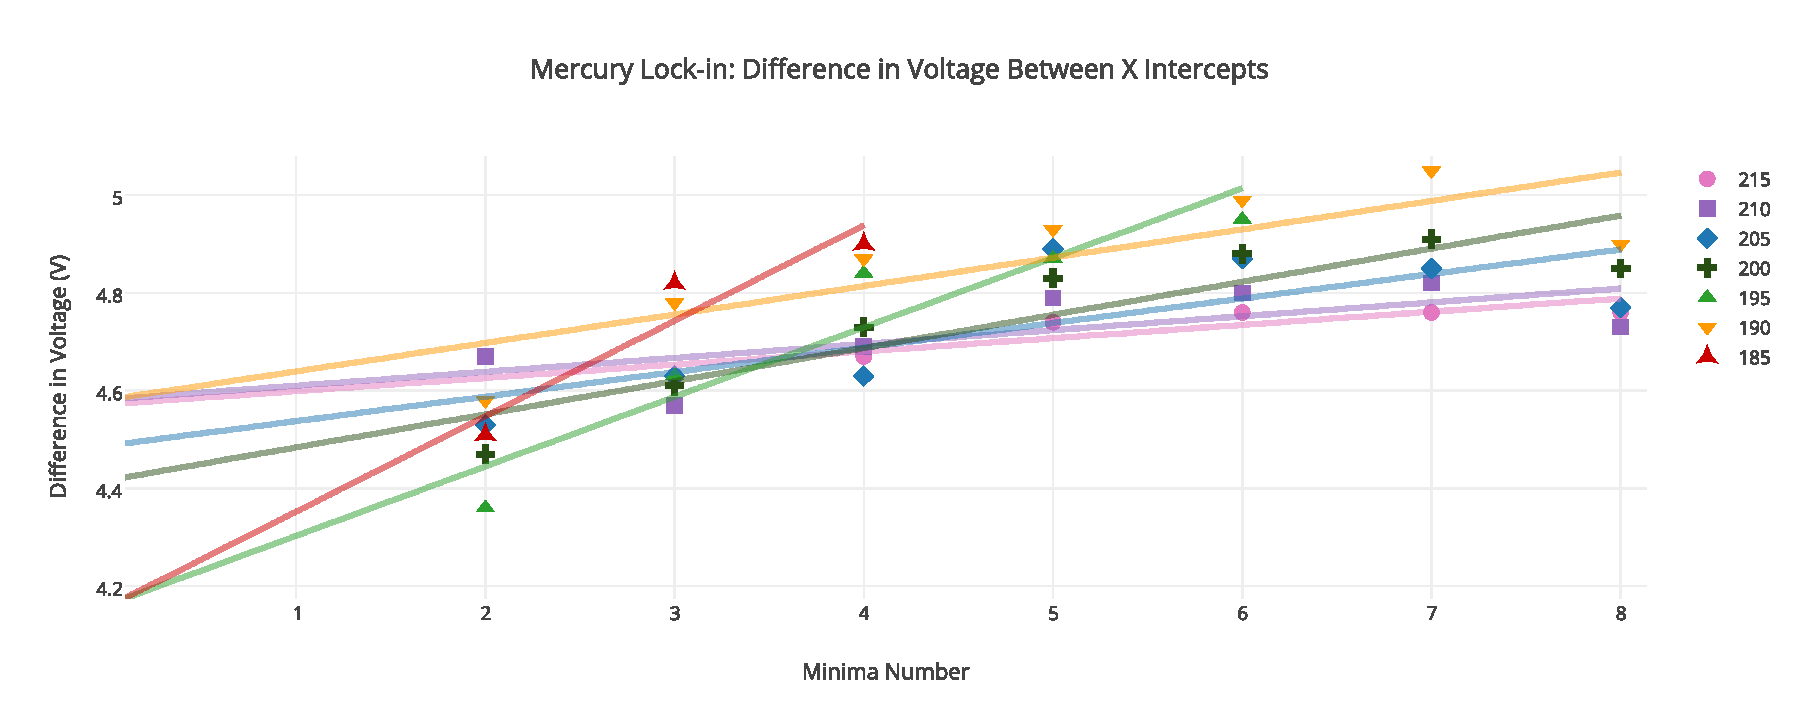
\includegraphics[width=6in]{lockin_intercepts.pdf}
\caption{The plot of the difference in voltage between minima versus the number of the minimum. All values have an uncertainty of ~1.3$\%$. The lines are linear fits to the data for each temperature. The two fits with steeper slopes correspond to the 195$^{\circ}$C and 185$^{\circ}$C data sets which were truncated due to ionization.}

\label{lockin_intercepts}
\end{figure}

The results of Table~\ref{hg_lockin_table} are plotted in Figure~\ref{lockin_intercepts}. Following the analysis outlined by Rapior, Sengstock and Baev, we used our fit lines to extrapolate to the voltages corresponding to a minima number of .5. Averaging these values gave us 4.46 $\pm$ .12 V where the uncertainty is the standard deviation of the mean. We repeated this analysis for all lock-in and direct data. The results obtained from all of our mercury data are in Table~\ref{hg_results}, note the much larger uncertainties for the direct output data than the lock-in data.  


\begin{table}[h!]
\centering
\caption{A summary of the best values and uncertainties from each of our data sets. All of these values, except the lock-in positive x-intercept value, agree with the expected energy value for mercury transitions.}
\begin{ruledtabular}
\begin{tabular}{c c c c}
 Direct Steepest Slope & Lock-in Minima & Direct Minima & Lock-in Positive Slope X-Intercept   \\
\hline	% horizontal line to separate headings from data

 4.6 $\pm$ 0.7 & 4.58 $\pm$ 0.24 V & 4.6 $\pm$ 0.4 & 4.46 $\pm$ 0.12 V  \\

\end{tabular}
\end{ruledtabular}
\label{hg_results}
\end{table}

Averaging the best values from each set of data, from Table~\ref{hg_results}, we got a final value of 4.56 $\pm$ .4 V. This value agrees with the known value of the lowest excitation $6^{1}S_{0}$ to $6^{3}P_{0}$ (4.67 eV) of mercury and also with the second excitation $6^{1}S_{0}$ to $6^{3}P_{1}$ (4.89 eV.)~\cite{newfeatures}

\section{Discussion}

All of our data was consistent with our expectations based on theory and past experiments. We were able to see the drops in electron current at regular intervals as electron gained enough energy to excite the neon or mercury atoms. For mercury, we saw that there was an optimal temperature range when drops in electron current were maximized in number and still discernible in amplitude. As suggested by Rapior,  Sengstock, and Baev, the difference in voltage between our minima tended to increase as the number of the minimum increased. 

Our final values for the energy needed to excite mercury show a stark trade off of accuracy versus precision. Our direct data values have a very large uncertainty (10 - 15$\%$), see Table~\ref{hg_results}, so they are not very precise, but they are accurate. Whereas our lock-in x-intercept data has a much smaller uncertainty (~2.7$\%$) a much higher precision, but it is no longer accurate because it is not in agreement with the known value of the excitation energy.

One of the biggest limitations in our experiment was our uncertainty in the precise voltages corresponding to the minima and steepest slopes. Particularly for the lock-in data, but also for the direct data, our uncertainty was largely based on the resolution of our graphs. The direct output data used the power supply that came with the apparatus, it had a resolution of 0.1 V. For the lock-in data we used an independent power supply that also increased the accelerating voltage in increments of 0.1 V. These increments of 0.1 V gave us an uncertainty on that order of magnitude and set a lower limit on our uncertainty. If we had increased the accelerating voltage in increments of 0.01 V, we would have had better resolution of our data and less uncertainty in our analysis. 

\section{Conclusion}

18.5 $\%$ .4 V, the value we got for the neon excitation energy, is in agreement with a large number of excitation energies for neon between 18.3 - 18.9 V. We were not able determine the energy transitions more precisely from the data that we collected. With our apparatus we were only able to obtain three minima before the neon ionized. Using different instrumentation we might be able to obtain more data and calculate the transition more precisely.

Our final value for mercury energy transitions was 4.56 $\pm$ .4 V which agrees with the known values for both the lowest energy transition, 4.67 eV, and the next lowest energy transition, 4.89 eV. We would hope for a more precise answer that would correspond with just one of the energy transitions. However, the resolution of our data was restricted by the apparatus we used.

It is possible that a most sensitive measurement of electron current we could have seen more minima below the first minima that we could detect. Having more minima would increase the number of data points used to fit lines and extrapolate the transition energy. Since some of our fit lines were made with only a couple of data points, increasing the number of points would help to average out outliners that are undiscernable with only a few points. 

Despite our difficulty in precisely determining the excitation energy of mercury, the overall results of this experiment are still as fascinating as they were for Franck and Hertz. This experiment clearly shows that electrons must have a certain quantified amount of energy before they can excite atoms. This result supports the premise of quantum mechanics and makes an abstract theory more tangible.

\begin{thebibliography}{9}


\bibitem{newfeatures} Gerald Rapior, Klaus Sengstock, and Valery Baev, "New Features of the Franck-Hertz Experiment,"  Am. J. Phys. \textbf{74}, 423--428 (2006). 

\bibitem{melissanos} Adrian C. Melissanos and Jim Napoitano, \textit{Experiments in Modern Physics} 2nd edition (Academic Press, Boston, 2003).

\bibitem{hyperphysics} Hyper-Physics: Franck-Hertz Experiment Website \url{<http://hyperphysics.phy-astr.gsu.edu/hbase/frhz.html>}

\end{thebibliography}


\end{document}
